\section{The measurement problem and the supply relation}\label{sec:03-framework}

Every method in this chapter infers market power from the way prices and quantities respond to observable shifts in
demand and cost. This section sets up the framework they share. It defines the objects we want to measure and writes
the supply relation that all later methods use. It then shows that an unrestricted conduct parameter fits any data,
explains with \citet{Stigler1964} why market structure alone cannot settle the question, and closes with a map of the
approaches.

\subsection{What we want to measure}\label{sec:03-objects}

Our main object is the \emph{Lerner index} $L = \frac{P - MC}{P}$, the gap between price and marginal cost as a share
of price (\cref{def:01-market-power}). A closely related object is the \emph{markup rate} $\frac{P - MC}{MC}$, the gap
as a share of marginal cost. The two carry the same information. A price 25 percent above marginal cost has a markup
rate of 0.25 and a Lerner index of $\frac{0.25}{1.25} = 0.2$. Both measure margins at the margin. They are not
measures of profit. Consider a firm with constant marginal cost $c$ and fixed cost $F$ that just breaks even under free
entry. It sets $P = c + \frac{F}{q}$, so its markup rate is $\frac{F}{cq} > 0$ although it earns no rents
(\cref{sec:01-fixed-costs}). A positive Lerner index measures the ability to price above marginal cost. Whether that
ability yields excess profits depends on fixed and sunk costs, which the methods of this chapter do not measure. The
same distinction runs through the recent debate on rising markups \citep{DeLoeckerEeckhoutUnger2020}, which
\cref{sec:01-rising-markups} reviews.

Two pricing rules from \cref{ch:theory} serve as benchmarks, the Lerner rule \eqref{eq:02-lerner} and
\cref{prop:02-cowling-waterson}. A monopolist with constant marginal cost $c$ facing demand $Q(P)$ with elasticity
$\varepsilon = -Q'(P)\frac{P}{Q(P)} > 0$ sets
\begin{equation*}
P - c = -\frac{Q(P)}{Q'(P)}, \qquad \frac{P - c}{P} = \frac{1}{\varepsilon}.
\end{equation*}
With $N$ Cournot firms, constant marginal costs $c_i$ and output shares $s_i = \frac{q_i}{Q}$, each firm satisfies
\begin{equation*}
\frac{P - c_i}{P} = \frac{s_i}{\varepsilon}, \qquad \sum_{i=1}^{N} s_i\,\frac{P - c_i}{P} = \frac{\HHI}{\varepsilon},
\end{equation*}
where $\HHI = \sum_i s_i^2$ is the Herfindahl index. Both rules are special cases of a single equation.

\begin{definition}[Supply relation and conduct parameter]\label{def:03-supply-relation}
Let $P(Q, Y)$ be inverse market demand, with demand shifters $Y$ and slope
$P'(Q, Y) \equiv \frac{\partial P(Q, Y)}{\partial Q} < 0$. Let $MC(Q, W)$ be industry marginal cost, with cost
shifters $W$. The \emph{supply relation} is
\begin{equation}\label{eq:03-supply-relation}
P = MC(Q, W) - \theta\, Q\, P'(Q, Y),
\end{equation}
and the number $\theta \ge 0$ is the \emph{conduct parameter}.
\end{definition}

Equation \eqref{eq:03-supply-relation} says that marginal cost equals a \emph{perceived marginal revenue}
$P + \theta Q P'$. We call it a supply relation because, outside perfect competition, firms do not have supply curves
that give output as a function of price alone \citep[p.~1016]{Bresnahan1989}. Dividing
\eqref{eq:03-supply-relation} by $P$ and using $\varepsilon = -\frac{P}{Q P'}$ gives the Lerner form
\begin{equation}\label{eq:03-lerner-theta}
\frac{P - MC}{P} = -\frac{\theta\, Q\, P'}{P} = \frac{\theta}{\varepsilon}
\qquad\Longleftrightarrow\qquad
\theta = \varepsilon\,\frac{P - MC}{P} \equiv L_\varepsilon .
\end{equation}
The conduct parameter is the \emph{elasticity-adjusted Lerner index} $L_\varepsilon$. It equals 0 under price taking,
$\frac{1}{N}$ under symmetric Cournot competition, and 1 under monopoly or joint profit maximization. Bertrand
competition with a homogeneous good and constant marginal cost gives $\theta = 0$ for any $N \ge 2$. It is also
convenient to name the \emph{markup term}
\begin{equation*}
m \equiv \frac{Q}{\left\lvert \frac{\partial Q}{\partial P}\right\rvert} = -Q\,P'(Q, Y) = \frac{P}{\varepsilon},
\end{equation*}
so that \eqref{eq:03-supply-relation} reads $P = MC + \theta m$. At $\theta = 1$, $m$ is the dollar markup of a
monopolist.

Industry data rarely come with firm-level costs and quantities. The next result shows what an industry-level
$\theta$ means when firms differ in costs and in conduct. It restates \cref{prop:02-theta-aggregate} with market
subscripts and generalizes \cref{prop:01-supply-relation}, which uses output shares as weights and constant conjectures.

\begin{proposition}[Aggregation of firm supply relations]\label{prop:03-aggregation}
Let $N$ firms produce a homogeneous good, with outputs $q_{it}$, industry output $Q_t = \sum_i q_{it}$, shares
$s_{it} = \frac{q_{it}}{Q_t}$ and market elasticity $\varepsilon_t = -\frac{P_t}{Q_t P'(Q_t)}$. Suppose each firm
satisfies the firm supply relation
\begin{equation*}
P_t = MC_{it} - \tilde\theta_{it}\, q_{it}\, P'(Q_t),
\end{equation*}
with firm-level conduct parameter $\tilde\theta_{it} \ge 0$. Then for any weights $\varphi_{it} \ge 0$ with
$\sum_i \varphi_{it} = 1$,
\begin{equation}\label{eq:03-aggregation}
P_t = \sum_{i=1}^{N} \varphi_{it}\, MC_{it} + \frac{P_t}{\varepsilon_t}\sum_{i=1}^{N} \varphi_{it}\, s_{it}\,
\tilde\theta_{it}.
\end{equation}
The industry therefore satisfies \eqref{eq:03-supply-relation} with industry marginal cost
$MC_t = \sum_i \varphi_{it} MC_{it}$ and industry conduct $\theta_t = \sum_i \varphi_{it}\, s_{it}\,\tilde\theta_{it}$.
\end{proposition}

\begin{proof}
Multiply firm $i$'s supply relation by $\varphi_{it}$ and sum over firms. The left side becomes
$\sum_i \varphi_{it} P_t = P_t$ because the weights sum to one. The right side becomes
\begin{align*}
\sum_i \varphi_{it} MC_{it} - P'(Q_t) \sum_i \varphi_{it}\,\tilde\theta_{it}\, q_{it}
&= \sum_i \varphi_{it} MC_{it} - Q_t P'(Q_t) \sum_i \varphi_{it}\,\tilde\theta_{it}\, s_{it} \\
&= \sum_i \varphi_{it} MC_{it} + \frac{P_t}{\varepsilon_t} \sum_i \varphi_{it}\,\tilde\theta_{it}\, s_{it},
\end{align*}
using $q_{it} = s_{it} Q_t$ in the first line and $-Q_t P'(Q_t) = \frac{P_t}{\varepsilon_t}$ in the second. Since
$\frac{P_t}{\varepsilon_t} = -Q_t P'(Q_t)$, equation \eqref{eq:03-aggregation} is \eqref{eq:03-supply-relation} with
the stated $MC_t$ and $\theta_t$.
\end{proof}

\begin{corollary}[Benchmarks for industry conduct]\label{cor:03-benchmarks}
Under the assumptions of \cref{prop:03-aggregation}, the following hold.
\begin{enumerate}[label=(\roman*)]
\item Cournot conduct ($\tilde\theta_{it} = 1$) gives $\theta_t = \sum_i \varphi_{it} s_{it}$. This equals
  $\frac{1}{N}$ for symmetric firms and $\HHI_t$ when $\varphi_{it} = s_{it}$.
\item Joint profit maximization gives $\tilde\theta_{it} = \frac{Q_t}{q_{it}} = \frac{1}{s_{it}}$ and hence
  $\theta_t = 1$ for any weights.
\item Price taking ($\tilde\theta_{it} = 0$) gives $\theta_t = 0$.
\item A constant conjectural variation $r_i = \frac{\dd Q_{-i}}{\dd q_i}$ gives $\tilde\theta_{it} = 1 + r_i$.
\end{enumerate}
\end{corollary}

\begin{proof}
Parts (i), (iii) and (iv) follow by substitution in $\theta_t = \sum_i \varphi_{it} s_{it}\tilde\theta_{it}$, with
$\sum_i s_{it}^2 = \HHI_t$ and, for (iv), the first-order condition
$P + q_i P'(Q)(1 + r_i) = MC_i$ of \cref{prop:01-supply-relation}. For (ii), joint profit
$P(Q)Q - \sum_j C_j(q_j)$ has derivative $P + Q P'(Q) - MC_i$ with respect to $q_i$. Setting it to zero and writing
$Q P' = \frac{Q}{q_i}\, q_i P'$ gives the firm supply relation with $\tilde\theta_{it} = \frac{Q_t}{q_{it}}$. Then
$\varphi_{it} s_{it} \tilde\theta_{it} = \varphi_{it}$, and the weights sum to one.
\end{proof}

\begin{remark}[Industry conduct is average conduct]\label{rem:03-average-conduct}
\Cref{prop:03-aggregation} says that an industry supply relation estimated on aggregate data measures a weighted
average of firms' marginal costs and a weighted average of their conduct. The weights are a choice of the analyst.
With $\varphi_{it} = s_{it}$ we recover the share-weighted margins of \citet{CowlingWaterson1976}. Firms with
different costs have different margins under most oligopoly models, so a stable industry marginal cost curve need not
exist. \citet[p.~1030]{Bresnahan1989} therefore reads the aggregate $\theta_t$ as industry average conduct. He rejects
the claim that oligopoly theory forces all firms to share the same conduct parameter. The electricity study in
\cref{sec:03-electricity} uses weights built from plant-level marginal costs and relies on this proposition.
\end{remark}

\begin{remark}[The language of conjectures]\label{rem:03-cv-language}
Much of the empirical literature writes $\tilde\theta_{it} = 1 + r_i$ and calls $r_i$ a \emph{conjectural variation},
the response of rivals' output that firm $i$ ``expects''. The two parameterizations are identical as a matter of logic
\citep[p.~1027]{Bresnahan1989}. The expectations reading is misleading near collusion. In repeated-game models of
tacit collusion, firms produce their collusive quotas because they expect a deviation to trigger a breakdown of
restraint (\cref{ch:collusion-theory}). Matching of a deviation is never observed in equilibrium. An estimated
``conjecture'' therefore measures how close behavior is to the collusive outcome. It says nothing about what rivals
would do after a deviation \citep[pp.~1028--1029]{Bresnahan1989}. \Cref{sec:01-cv-warning} develops the point.
\end{remark}

\subsection{An unrestricted conduct parameter has no content}\label{sec:03-content}

The supply relation becomes a model only once we restrict how conduct varies. To see why, index markets or firms by
$i$ and periods by $t$, and allow conduct to vary freely:
\begin{equation}\label{eq:03-general-model}
P_{it} = mc_{it} + \theta_{it}\,\frac{Q_{it}}{\left\lvert \frac{\partial Q_{it}}{\partial P_{it}}\right\rvert}.
\end{equation}
The absolute value matters. The demand slope is negative, so dividing $Q_{it}$ by the slope itself would turn the
markup term into a markdown.

\begin{proposition}[Exact fit]\label{prop:03-exact-fit}
Take any data $\{(P_{it}, Q_{it})\}$, any demand slopes $\frac{\partial Q_{it}}{\partial P_{it}} < 0$ and any marginal
cost function $mc_{it} = c(q_{it}, W_{it}; \beta)$ with any parameter $\beta$. Then
\begin{equation*}
\theta_{it} = \frac{(P_{it} - mc_{it})\left\lvert \frac{\partial Q_{it}}{\partial P_{it}}\right\rvert}{Q_{it}}
\end{equation*}
satisfies \eqref{eq:03-general-model} exactly at every observation.
\end{proposition}

This is \cref{prop:02-theta-fit}, restated because every method below responds to it. The proposition has a
sharp implication. With as many conduct parameters as observations, the model needs no error
term and rejects nothing, whatever functional form we impose on cost. The $\theta_{it}$ absorb every residual. Empirical
content comes only from restrictions on conduct. Four kinds appear in this chapter.
\begin{enumerate}[label=(\alph*)]
\item Conduct is constant, or constant within a small number of regimes such as collusion and price wars.
\item Conduct lies in $[0, 1]$, which bounds marginal cost between $P_{it} + Q_{it}P'(Q_{it})$ and $P_{it}$.
\item Conduct is uncorrelated with the instruments used to estimate it.
\item Conduct takes the value implied by a specific game, such as Cournot or joint profit maximization.
\end{enumerate}
Every method below combines one or more of these restrictions with restrictions on demand and cost. Restriction (b)
alone yields bounds (\cref{sec:03-bounds}). \Cref{sec:03-corts} shows what an estimated constant $\theta$ measures
when restriction (a) fails \citep{Corts1999}.

\subsection{Why structure does not pin down conduct: Stigler (1964)}\label{sec:03-stigler}

The structure-conduct-performance tradition took conduct to follow from structure. \citet{Stigler1964} gave the first
systematic argument for why it need not. \Cref{sec:02-stigler} develops his model, his four detection criteria and his
evidence in full, with the original tables. Here we keep the part of the argument that bears on measurement.

\casehead{The policing problem}
Stigler started from the premise that oligopolists wish to collude to maximize joint profits. He asked why collusion
succeeds in some markets and fails in others. His answer is that a collusive agreement must be policed. Any member who
can cut prices secretly earns more than by conforming. The basic evidence of a secret cut is that the cutter wins
customers it would otherwise not obtain. Policing is therefore a problem of statistical inference from sales.

In his model, $n_s$ sellers of equal size share $n_o$ old buyers. Each old buyer returns to his supplier with
probability $\phi$, as in \cref{sec:02-stigler}, and otherwise moves to one of the other sellers at random. A seller
observes only its own sales. It suspects a rival of price cutting when its own losses of old customers and the rival's
gains are both improbably large. Stigler's Criterion I \eqref{eq:02-stigler-crit1} gives the largest share of average
sales that a price cutter can take from one rival without detection. It falls with the number of buyers and with the
repeat probability, and it barely depends on the number of sellers (\cref{tab:02-stigler-t1}). With 100 old buyers, 10
sellers and $\phi = 0.9$, a firm can take 5.4 percent of average sales from each rival. That is about 50 percent from all
nine together. If the nine rivals merge or pool their information, the gain falls to 28.5 percent (Panel C of
\cref{tab:02-stigler-t234}).

The model also yields a concentration measure. If each new buyer chooses a seller with probability equal to its market
share, the sampling noise that masks secret cuts is proportional to $1 - \HHI$ \eqref{eq:02-stigler-hhi}. The Herfindahl
index thus emerges from the detection problem itself. Collusion is harder to sustain with more sellers, more and smaller
buyers, more turnover among buyers and more new buyers. It is easier with unequal sellers and against buyers who reveal
the prices they pay. \citet{GreenPorter1984} later formalized secret price cutting as a repeated game with imperfect
monitoring, in which price wars occur on the equilibrium path (\cref{ch:collusion-theory}).

\casehead{Evidence}
Stigler's own evidence is fragmentary. Newspaper advertising rates in 1939 and radio spot rates in 1961 respond little to
the number of rival sellers (\cref{tab:02-stigler-t56}). Across 17 industries, all six rank correlations between
profitability and concentration are positive (\cref{tab:02-stigler-t7}). The Herfindahl index correlates more strongly
with profitability than the four-firm share does. Stigler nonetheless finds no relation when $\HHI$ is below 0.25 or the
four-firm share below about 80 percent. Among steel products in 1939, discounts from list prices are larger where the
Herfindahl index is smaller, with a rank correlation of $-0.55$ (\cref{tab:02-stigler-t9}). Stigler called this evidence
``fairly favorable to the theory'' and added that it did not constitute strong support.

\casehead{Lessons for measurement}
In Stigler's model the map from structure to conduct depends on what sellers can observe. It also depends on the
number, size and turnover of buyers, and on the dynamics of detection and punishment. None of these is captured by
a concentration ratio. Two markets with the same Herfindahl index can therefore support very different conduct. This is
the deepest reason why the methods of this chapter measure conduct industry by industry.

Cross-sections of prices and concentration face further problems of interpretation \citep[pp.~1042--1044]{Bresnahan1989}.
Concentration is endogenous. Under free entry, larger markets hold more firms, and price equals average cost
everywhere, so a price-concentration relation need not reflect conduct. With heterogeneous costs, markets with more firms
offer more draws on a low-cost firm (\cref{prop:01-more-draws}). In the aggregate supply relation of
\cref{prop:03-aggregation}, a lower price in unconcentrated markets may reflect lower average marginal cost, lower average
conduct, or both. \Cref{sec:01-price-concentration} treats these studies in detail.

\subsection{A taxonomy of approaches}\label{sec:03-taxonomy}

\Cref{tab:03-taxonomy} organizes the approaches of this chapter by the data they need, the assumptions they maintain and
what they deliver. Some deliver tests of a single hypothesis, some deliver bounds, and some deliver point estimates of
$\theta$. \Cref{tab:01-id-strategies} gives a complementary classification by identification argument.

\begin{table}[!htb]
\centering
\begin{threeparttable}
\caption{Approaches to measuring market power in homogeneous-goods industries}
\label{tab:03-taxonomy}
\footnotesize
\setlength{\tabcolsep}{3.5pt}
\begin{tabularx}{\textwidth}{@{}>{\raggedright\arraybackslash}p{2.3cm}
  >{\raggedright\arraybackslash}X >{\raggedright\arraybackslash}X >{\raggedright\arraybackslash}X
  >{\raggedright\arraybackslash}p{1.5cm}@{}}
\toprule
Approach & Data needed & Maintained assumptions & What is identified & Section \\
\midrule
(a) Market-wide cost shifters & Prices and an observed, exogenous cost component (taxes). Quantities or revenue for
  some tests & Shape of demand and of marginal cost. Long-run equilibrium for the revenue test & Test of competition.
  Bounds on $\theta$. Sign of the revenue statistic & \ref{sec:03-sumner}, \ref{sec:03-revenue-tests} \\
\addlinespace
(b) Firm-specific cost shifters & One firm's price and quantity, its own cost shifters and rivals' cost shifters & Own
  cost shifters excluded from rivals' supply. Special conduct for a markup reading & Slope of the firm's residual
  demand & \ref{sec:03-residual-demand} \\
\addlinespace
(c) Demand rotations & Industry price and quantity, a demand shifter, a demand rotator and cost shifters & Functional
  forms of demand and marginal cost. Constant $\theta$ & Point estimate of $\theta$ and of the slope of marginal cost &
  \ref{sec:03-identification} \\
\addlinespace
(d) Observed marginal cost & Prices, quantities and engineering or accounting cost data & Correct measurement of
  marginal cost. Estimated demand elasticity & $\theta_t = \varepsilon_t L_t$ observation by observation. Validation
  of (c) & \ref{sec:03-sugar}, \ref{sec:03-electricity} \\
\addlinespace
(e) Cost and factor-demand functions & Prices, output, factor prices, input quantities & Flexible cost function
  homogeneous of degree one in factor prices. Correct price of capital & Marginal cost from factor demands, then
  $\theta$ & \ref{sec:03-taxonomy} \\
\addlinespace
(f) Regime switching & Long time series of price and quantity & Two or more conduct regimes. No other unobserved
  shifts of the supply relation & Size and frequency of shifts in conduct & \cref{ch:collusion-evidence} \\
\bottomrule
\end{tabularx}
\begin{tablenotes}\footnotesize
\item Notes: Our construction. Approach (a) covers \citet{Sumner1981}, \citet{Sullivan1985},
\citet{AshenfelterSullivan1987} and \citet{PanzarRosse1987}. Approach (b) is \citet{BakerBresnahan1988}, and (c) is
\citet{Bresnahan1982} and \citet{Lau1982}. Approach (d) covers \citet{GenesoveMullin1998} and \citet{Wolfram1999}.
Approach (e) covers \citet{GollopRoberts1979}, \citet{Appelbaum1979,Appelbaum1982} and \citet{Hall1988}, and (f) is
\citet{Porter1983}.
\end{tablenotes}
\end{threeparttable}
\end{table}

Approach (e) gets no section of its own, so we describe it here. Let $w = (w_1, \dots, w_K)$ be the vector of factor
prices, as in \cref{sec:03-panzar-rosse}. The approach estimates marginal cost from a flexible cost function $C(Q, w)$
and its factor demands $X_k = \frac{\partial C}{\partial w_k}$ (Shephard's lemma, \cref{app:math}). It estimates them
jointly with demand and the supply relation \citep[Section~3.3]{Bresnahan1989}. Its identifying idea is homogeneity
\citep[p.~1034]{Bresnahan1989}. Total cost is homogeneous of degree one in factor prices, so marginal cost is too, and
Euler's theorem gives
\begin{equation*}
MC(Q, w) = \sum_{k} w_k\,\frac{\partial MC(Q, w)}{\partial w_k}.
\end{equation*}
Every term of marginal cost therefore scales with factor prices, while the markup term $\theta m$ in $P = MC + \theta m$
does not. Scaling all factor prices by a common factor moves marginal cost proportionally and leaves the markup term
unchanged. Any part of the supply relation that does not scale with factor prices is attributed to market power.
\Cref{sec:01-id-demand} gives a worked example. The approach leans hard on the functional form of cost and on observing
the true marginal price of every input. Valuing capital services is the familiar weak point, and it revives the
accounting critiques of the cross-industry literature \citep[p.~1040]{Bresnahan1989}.

\section{Testing with cost pass-through: Sumner (1981)}\label{sec:03-sumner}

Suppose one component of marginal cost is observed and varies for reasons unrelated to demand. Then the response of
price to that component reveals the pricing rule, without any measurement of the rest of cost. Excise taxes are such
a component. \citet{Sumner1981} used state cigarette taxes to test whether the US cigarette industry behaved
competitively, collusively, or in between. This section first develops the theory of pass-through under general conduct.
It then presents Sumner's design and results, the critiques his test invites, and a replication that clarifies what the
data can and cannot reveal.

\subsection{Pass-through under conduct}\label{sec:03-passthrough-theory}

\begin{assumption}[Pass-through environment]\label{ass:03-passthrough}
A homogeneous good has twice differentiable inverse demand $P(Q)$ with $P'(Q) < 0$. Industry marginal cost $MC(Q)$ is
differentiable with $MC'(Q) \ge 0$. A specific (per-unit) tax $t$ is collected from sellers, so effective marginal cost
is $MC(Q) + t$. Conduct $\theta \ge 0$ does not vary with $t$, and the equilibrium is interior and satisfies the supply
relation
\begin{equation}\label{eq:03-supply-tax}
P(Q) + \theta\, Q\, P'(Q) = MC(Q) + t .
\end{equation}
\end{assumption}

Three local features of the primitives govern pass-through. The \emph{curvature} of inverse demand is
$\chi \equiv -\frac{Q P''(Q)}{P'(Q)}$. It is zero for linear demand and positive when inverse demand is convex. The
price elasticity of demand is $\varepsilon = -\frac{P}{Q P'(Q)}$. The elasticity of the effective marginal cost curve
is $\varepsilon_S \equiv \frac{MC + t}{Q\, MC'(Q)}$, which is infinite when marginal cost is flat. \emph{Pass-through}
is $\rho \equiv \frac{\dd P}{\dd t}$, the change in the equilibrium price per unit change in the tax.

\begin{proposition}[Pass-through under conduct]\label{prop:03-passthrough}
Under \cref{ass:03-passthrough}, let $J \equiv P'(1 + \theta) + \theta Q P'' - MC'$ and suppose the stability condition
$J < 0$ holds. \Cref{prop:02-pt-general} then gives
\begin{equation}\label{eq:03-passthrough-general}
\rho = \frac{1}{1 + \theta(1 - \chi) + \frac{MC'(Q)}{\lvert P'(Q)\rvert}}
     = \frac{1}{1 + \frac{\theta}{\varepsilon_{ms}} + \frac{\varepsilon - \theta}{\varepsilon_S}},
\qquad \varepsilon_{ms} \equiv \frac{1}{1 - \chi},
\end{equation}
and both denominators are positive.
\end{proposition}

The stability condition $J < 0$ is the condition $\Lambda < 0$ of \cref{ass:02-pt-general}, written out with
$ms' = -P'(1 - \chi)$. It says that perceived marginal revenue cuts effective marginal cost from above. Differentiating
\eqref{eq:03-supply-tax} in $t$ gives $\frac{\dd Q}{\dd t} = \frac{1}{J} < 0$, so output falls when the tax rises. The
price moves along the demand curve, so $\rho = \frac{P'}{J}$, and dividing by $P'$ gives the first form. Steps 4 and 5 of
the proof of \cref{prop:02-pt-general} show that $\frac{MC'}{\lvert P'\rvert} = \frac{\varepsilon - \theta}{\varepsilon_S}$,
which links the two forms.

The second form in \eqref{eq:03-passthrough-general} is the formula of \citet[eq.~(2), p.~548]{WeylFabinger2013} for
constant conduct. They call $\varepsilon_{ms} = \frac{ms}{Q\, ms'}$, with $ms(Q) = -QP'(Q)$, the elasticity of the
inverse marginal surplus function \citep[p.~538]{WeylFabinger2013}. Their formula adds the term
$\frac{\theta}{\varepsilon_\theta}$ to the denominator, where $\varepsilon_\theta = \frac{\theta}{Q\,\theta'(Q)}$ is the
elasticity of conduct with respect to output (\cref{sec:02-pt-general}). The term vanishes here because $\theta$ is
constant.

\begin{corollary}[Special cases]\label{cor:03-passthrough-cases}
\Cref{cor:02-pt-cases}, \cref{cor:02-bulow-pfleiderer} and \cref{ex:02-pt-examples} give the following special cases
of \cref{prop:03-passthrough}.
\begin{enumerate}[label=(\roman*)]
\item Competition with rising marginal cost ($\theta = 0$) gives
  $\rho = \frac{1}{1 + \frac{\varepsilon}{\varepsilon_S}} = \frac{\varepsilon_S}{\varepsilon_S + \varepsilon} \le 1$,
  with equality only when marginal cost is flat (\cref{cor:02-pt-cases}(i)).
\item Monopoly with flat marginal cost gives $\rho = \frac{1}{2 - \chi}$. In terms of direct demand $D(P)$,
  $\chi = \frac{D(P) D''(P)}{D'(P)^2}$, so $\rho < 1$ if and only if $D$ is log-concave
  (\cref{lem:02-chi-direct,cor:02-bulow-pfleiderer}).
\item Linear demand ($\chi = 0$) with flat marginal cost gives $\rho = \frac{1}{1 + \theta}$
  (\cref{ex:02-pt-examples}(i)).
\item Constant-elasticity demand $P = A Q^{-\frac{1}{\varepsilon}}$ has $\chi = 1 + \frac{1}{\varepsilon}$, and with
  flat marginal cost $\rho = \frac{\varepsilon}{\varepsilon - \theta}$ (\cref{ex:02-pt-examples}(iii)).
\item The Bulow-Pfleiderer family $P = a - bQ^{\gamma}$, with $b, \gamma > 0$, has $\chi = 1 - \gamma$, and with flat
  marginal cost $\rho = \frac{1}{1 + \theta\gamma}$ (\cref{ex:02-pt-examples}(ii)).
\item Log demand $P = a - b\ln Q$, with $b > 0$, has $\chi = 1$, and with flat marginal cost $\rho = 1$ for every
  $\theta$. The markup is the constant $\theta b$ (\cref{ex:02-pt-examples}(iv)).
\end{enumerate}
The symbols $A$, $a$, $b$ and $\gamma$ are local to this corollary.
\end{corollary}

Part (v) is the family of \cref{ex:02-bp} in inverse form, with $\gamma = \frac{1}{g}$. \Cref{sec:03-sugar} writes it
in direct form, as \citet{GenesoveMullin1998} do, so the exponent there is the reciprocal of the $\gamma$ used here.
The log demand of part (vi) is the inverse of exponential direct demand $Q = e^{\frac{a - P}{b}}$.

\Cref{fig:03-passthrough-curves} plots pass-through against conduct for four demand curves with flat marginal cost.
Under competition every curve passes through $\rho = 1$. As conduct rises, the curves fan out in a direction set by
curvature alone. Pass-through exceeds one only for demand more convex than log demand.

\begin{figure}[htbp]
\centering
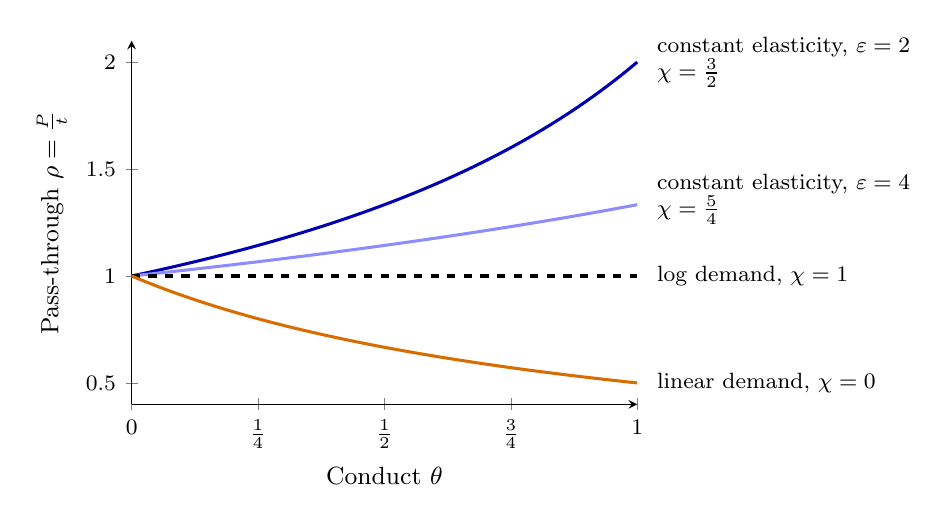
\begin{tikzpicture}
\begin{axis}[
  width=0.66\textwidth, height=6.2cm,
  xmin=0, xmax=1, ymin=0.4, ymax=2.1,
  xlabel={Conduct $\theta$}, ylabel={Pass-through $\rho = \frac{\dd P}{\dd t}$},
  xtick={0,0.25,0.5,0.75,1}, ytick={0.5,1,1.5,2},
  xticklabels={$0$,$\frac{1}{4}$,$\frac{1}{2}$,$\frac{3}{4}$,$1$},
  tick label style={font=\footnotesize}, label style={font=\small},
  axis lines=left, clip=false, every axis plot/.append style={line width=1.1pt}]
  \addplot[domain=0:1, samples=60, color=blue!70!black] {2/(2-x)};
  \addplot[domain=0:1, samples=60, color=blue!45] {4/(4-x)};
  \addplot[domain=0:1, samples=2, color=black, dashed] {1};
  \addplot[domain=0:1, samples=60, color=orange!85!black] {1/(1+x)};
  \node[anchor=west, font=\footnotesize, align=left] at (axis cs:1.02,2.0)
    {constant elasticity, $\varepsilon = 2$\\ $\chi = \frac{3}{2}$};
  \node[anchor=west, font=\footnotesize, align=left] at (axis cs:1.02,1.36)
    {constant elasticity, $\varepsilon = 4$\\ $\chi = \frac{5}{4}$};
  \node[anchor=west, font=\footnotesize, align=left] at (axis cs:1.02,1.0)
    {log demand, $\chi = 1$};
  \node[anchor=west, font=\footnotesize, align=left] at (axis cs:1.02,0.5)
    {linear demand, $\chi = 0$};
\end{axis}
\end{tikzpicture}
\caption{Pass-through of a specific tax as a function of conduct for four demand curves, with flat marginal cost. From
\cref{cor:03-passthrough-cases}, $\rho = \frac{1}{1 + \theta(1 - \chi)}$. Linear demand gives $\frac{1}{1 + \theta}$,
log demand gives 1 for every $\theta$, and constant elasticity gives $\frac{\varepsilon}{\varepsilon - \theta}$. The
dashed line is also the competitive benchmark.}
\label{fig:03-passthrough-curves}
\end{figure}

\begin{proposition}[What pass-through identifies]\label{prop:03-passthrough-id}
\Cref{cor:02-pt-reveal} gives the following. Under \cref{ass:03-passthrough} with flat marginal cost, pass-through
identifies only the composite
\begin{equation}\label{eq:03-kappa}
\kappa \equiv \theta(\chi - 1) = 1 - \frac{1}{\rho}.
\end{equation}
Consequently, the following hold.
\begin{enumerate}[label=(\roman*)]
\item $\rho > 1$ rejects $\theta = 0$ for every demand curve. Rising marginal cost only strengthens the rejection.
\item Any $\rho$ in $(0, \infty)$ is consistent with every conduct $\theta \in (0, 1]$, for a suitable curvature.
  Pass-through alone never rejects monopoly.
\item Under constant-elasticity demand with elasticity $\varepsilon$, $\theta = \varepsilon\kappa$.
\end{enumerate}
\end{proposition}

Equation \eqref{eq:03-kappa} is \eqref{eq:02-pt-kappa}. Part (i) combines parts (i) and (iii) of
\cref{cor:02-pt-reveal}. Parts (ii) and (iii) are parts (ii) and (iv) of that corollary. Given $\rho$ and conduct
$\theta > 0$, the curvature $\chi = 1 + \frac{\kappa}{\theta}$ reproduces the observed pass-through.

The proposition is the key to reading every cost pass-through study. A market-wide cost shock moves the equilibrium
along a single demand curve. What it reveals is the slope of perceived marginal revenue relative to the slope of demand,
and that slope mixes conduct with curvature. Separating them needs either an assumption on curvature, as in Sumner's
constant elasticity, or variation that changes the slope of demand at a given point (\cref{sec:03-identification}).

\subsection{Sumner's design and results}\label{sec:03-sumner-design}

\casehead{The question}
Is the US cigarette industry competitive, collusive, or in between? The industry was a textbook example of oligopoly.
In the Tobacco Case of 1946 the major manufacturers were convicted of operating an illegal cartel, and the consensus
was that their behavior did not change after the verdict \citep[p.~1010]{Sumner1981}. Earlier work had measured market
power by the ratio of price to marginal cost, which requires cost data that are rarely reliable. Sumner proposed a
scheme that avoids measuring cost: ``The coefficient of the tax rate term in a price equation identifies the ratio of
price to marginal cost'' \citep[p.~1010]{Sumner1981}.

\casehead{The setting}
Cigarettes carry a federal excise tax and state excise taxes, both specific taxes per pack. The federal tax was 8 cents
per pack for more than 25 years. The median state tax rose from 3 cents in 1954 to 12 cents in 1978. Combined taxes
nonetheless fell in real terms, from 48.7 percent of the retail price in 1954 to 35.5 percent in 1978. In 1978 state
taxes ranged from 2 cents in North Carolina to 21 cents in Florida, Connecticut and Massachusetts. The three states with
a large stake in tobacco growing and cigarette manufacturing (North Carolina, Virginia and Kentucky) all had low taxes.
Tobacco interests cannot explain the variation among the other states \citep[n.~8]{Sumner1981}.

Two features of the distribution system matter for the test. First, the institutions limit arbitrage across states.
The federal tax is paid by manufacturers, with the stamp affixed at the factory. Distributors must hold a license in the
state where they operate and must pay the state tax and affix its stamp within a few days of receiving a shipment.
Reselling out of state requires a special permit. Manufacturers therefore know the final state of sale and could, in
principle, set prices that depend on the state tax. Sumner argues that differentials of several cents per pack could
persist before arbitrage became profitable. Second, he assumes that wholesale and retail distribution are competitive,
citing the large numbers of retailers and distributors in each market.

\casehead{The data}
The panel covers 47 states and the District of Columbia annually from 1954 to 1978, 1,200 state-years. Alaska, Hawaii
and New Hampshire are excluded for lack of data and peculiar tax laws. Prices are the Tobacco Tax Council's
``weighted-average price per package'' for each state and year. The Council asks wholesalers for average retail prices
by type of cigarette (regular, king, 100 mm) and type of sale (carton, single pack, machine). It aggregates them with
national weights, so the most obvious quality differences are held fixed across states.

\casehead{The model}
Sumner starts from the markup rule of a firm $j$ facing a demand curve with elasticity $\eta_j < 0$ (his sign
convention),
\begin{equation*}
P_j = \frac{\eta_j}{\eta_j + 1}\, M_j \qquad \text{(his eq.~1)},
\end{equation*}
where $M_j$ is marginal cost. In our notation, with $\varepsilon_j = -\eta_j > 0$, this is
$P_j = \frac{\varepsilon_j}{\varepsilon_j - 1} M_j$. Under monopoly $\varepsilon_j$ is the market elasticity, and under
perfect competition it is infinite. Marginal cost is expanded as $M_j = X_j\beta + e_j + R$ (his eq.~2), with observed
cost factors $X_j$, unobserved factors $e_j$ and the tax $R$, which does not vary by firm.

Only state-average prices are observed, so Sumner aggregates. Let $S_j$ be firm $j$'s market share, $\omega_j \equiv
\frac{P_j}{M_j}$ its price-to-cost ratio, and $P = \sum_j S_j P_j$, $M = \sum_j S_j M_j$ and
$\bar\omega = \sum_j S_j\omega_j$ the share-weighted averages. Then
\begin{equation*}
P = \sum_j S_j\,\omega_j M_j = \bar\omega M + \sum_j S_j(\omega_j - \bar\omega)(M_j - M) \qquad \text{(his eq.~3)}.
\end{equation*}
To verify the identity, expand the last sum. It equals $\sum_j S_j\omega_j M_j - \bar\omega M - \bar\omega M +
\bar\omega M$, because $\sum_j S_j = 1$. Sumner also identifies $\bar\omega$ with $\frac{\bar\eta}{\bar\eta + 1}$ for
the share-weighted elasticity $\bar\eta$, which holds only approximately because the map is nonlinear. The covariance
term vanishes if price-cost ratios or marginal costs vary little across firms, or are unrelated. Sumner argues that
retail prices vary little across brands within a market and that costs are similar, since cigarettes are made in one
region with a standard technology. Dropping the covariance term gives $P = \bar\omega M$, and substituting the cost
equation gives the linear price equation
\begin{equation*}
P_{it} = X_{it}\psi + \bar\omega R_{it} + U_{it} \qquad \text{(his eq.~4)},
\end{equation*}
with states $i$, years $t$, $\psi = \bar\omega\beta$ and $U_{it} = \bar\omega e_{it}$. Sumner calls the tax coefficient
$\theta$. Under constant $\bar\omega$ it equals the pass-through $\frac{\dd P}{\dd R}$, so we write it as $\rho$.

The link to conduct is direct. With constant-elasticity market demand, flat marginal cost and conduct $\theta$,
\cref{cor:03-passthrough-cases}(iv) gives $P = \frac{\varepsilon}{\varepsilon - \theta}(k + t)$, with non-tax marginal
cost $k$ and tax $t$. Comparing with his eq.~1, Sumner's firm-level elasticity is
\begin{equation*}
\varepsilon_j = \frac{\varepsilon}{\theta},
\end{equation*}
the market elasticity divided by conduct. It is the elasticity that firms behave as if they face.

\casehead{The estimating equation and the estimator}
With states indexed by $s$ and years by $y$, the most complete specification is
\begin{equation}\label{eq:03-sumner-regression}
p_{sy} = \mu_s + \tau_y + \rho\, t_{sy} + e_{sy}.
\end{equation}
Here $p_{sy}$ is the price per pack and $t_{sy}$ the combined state and federal tax. The terms $\mu_s$ and $\tau_y$ are
state and year fixed effects. The state effects absorb $\frac{\varepsilon}{\varepsilon - \theta}k_{sy}$ to the extent that it is
constant within a state, and the year effects absorb national cost and price-level changes. Equation
\eqref{eq:03-sumner-regression} is a two-way fixed-effects, or difference-in-differences, regression
(\cref{app:econometrics}). Sumner estimates it by OLS. He also reports a specification that replaces the year effects
by the national consumer price index and drops the state effects. He estimates it by OLS and by a variance-components
(random-effects) generalized least squares (GLS) estimator with random state and year effects
\citep{FullerBattese1974}.

The hypotheses are sharp. Competition with flat marginal cost implies $\rho = 1$. Monopoly with constant-elasticity
demand implies $\rho = \frac{\varepsilon}{\varepsilon - 1} > 1$, and conduct $\theta$ implies
$\rho = \frac{\varepsilon}{\varepsilon - \theta}$. An estimate of $\rho$ can be inverted for the firm-level elasticity,
$\varepsilon_j = \frac{\rho}{\rho - 1}$.

\casehead{Identification}
Tax variation is treated as exogenous: the residual $e_{sy}$ is assumed uncorrelated with $t_{sy}$ given the fixed
effects. The state effects absorb stable differences in tax levels, such as the low taxes of producing states. What
identifies $\rho$ is therefore the timing of tax changes within states relative to other states. The assumption fails
if states raise taxes when local costs or demand change, or if taxes shift the demand for legal sales through
cross-border shopping and smuggling. The tax shifts the marginal cost of every seller in a state by the same amount, so
the test concerns market demand and industry conduct. A cost shifter specific to one firm would instead trace out that
firm's residual demand (\cref{sec:03-residual-demand}).

\casehead{Results}
\Cref{tab:03-sumner} reproduces Sumner's Table 1. With state and year effects, $\hat\rho = 1.074$ with a standard
error of 0.013. A 10-cent difference in taxes thus raises the price by 10.74 cents. The $t$-statistic for $\rho = 1$ is
$\frac{1.074 - 1}{0.013} = 5.7$. The other two specifications give 1.029 and 1.069, with $t$-statistics of 2.6 and 5.3.
All three reject competition at conventional levels. The last column of the table reports our replication on a
reconstructed panel (\cref{sec:03-sumner-replication}), which reproduces all three estimates to within 0.001.

\begin{table}[htbp]
\centering
\begin{threeparttable}
\caption{Effect of the excise tax on the retail price of cigarettes}
\label{tab:03-sumner}
\small
\begin{tabular}{@{}lccccccc@{}}
\toprule
& \multicolumn{4}{c}{Sumner (1981), Table 1} & \multicolumn{2}{c}{Implications} & Replication \\
\cmidrule(lr){2-5}\cmidrule(lr){6-7}\cmidrule(l){8-8}
& $\hat\rho$ & Elasticity & Controls & Method & $t$ for $\rho = 1$ & $\frac{\hat\rho}{\hat\rho - 1}$ &
  $\hat\rho$ \\
\midrule
(1) & \makecell{1.074\\(0.013)} & $-13.5$ & $DY_t$, $DS_i$ & OLS & 5.7 & 14.5 & \makecell{1.075\\(0.013)} \\
\addlinespace
(2) & \makecell{1.029\\(0.011)} & $-34.5$ & NCPI & OLS & 2.6 & 35.5 & \makecell{1.029\\(0.011)} \\
\addlinespace
(3) & \makecell{1.069\\(0.013)} & $-14.5$ & NCPI & VC & 5.3 & 15.5 & \makecell{1.069\\(0.013)} \\
\bottomrule
\end{tabular}
\begin{tablenotes}\footnotesize
\item Notes: The dependent variable is the retail price per pack in cents. The sample has 1,200 state-years (48 states
including DC, 1954--78). Standard errors are in parentheses. ``Elasticity'' is Sumner's implied price elasticity, with his negative sign.
$DY_t$ are year dummies (1978 excluded) and $DS_i$ state dummies (Wyoming excluded). NCPI is the national consumer
price index, and row (2) has no state dummies. VC is a variance-components (random-effects) GLS estimator with a random
effect for each state and each year. Sumner reports $R^2$ of about 0.99 with dummies and about 0.95 without. Our
replication gives 0.994 and 0.985. The column $\frac{\hat\rho}{\hat\rho - 1}$ inverts his eq.~1 exactly, in absolute
value. The replication uses OLS for rows (1) and (2) and two-way random-effects GLS for row (3), with conventional
standard errors, as in the paper.
\end{tablenotes}
\end{threeparttable}
\end{table}

The implied elasticities in the table deserve a check. Sumner's reported values equal $\frac{1}{1 - \hat\rho}$
exactly, for example $\frac{1}{1 - 1.074} = -13.5$. Inverting his eq.~1 exactly instead gives
$\eta_j = -\frac{\hat\rho}{\hat\rho - 1}$, which is $-14.5$, $-35.5$ and $-15.5$. The reported values thus treat
$\hat\rho - 1$ as the markup over cost, $\frac{P - M}{M} = -\frac{1}{\eta_j}$, in place of the Lerner condition
$\frac{P - M}{P} = -\frac{1}{\eta_j}$. The two agree to first order in $\frac{1}{\lvert\eta_j\rvert}$, so the
difference is immaterial for his conclusions. His text uses the same approximation: ``Taking $\theta = 1.05$, a 1
percent rise in the price of a firm's product would cause a 20 percent fall in the quantity sold'' \citep[p.~1019]{Sumner1981}.

\casehead{Robustness}
Sumner reports four checks. First, he estimates nonlinear versions of eq.~4 that let the price-to-cost ratio vary with
price, $\bar\omega(P) = \gamma P^{1 - \lambda}$. Substituting in $P = \bar\omega(P) M$ gives $P^{\lambda} = \gamma M$,
which he estimates by nonlinear least squares with additive and multiplicative errors (his eqs.~4$'$ and 4$''$). The
hypothesis $\lambda = 1$, under which the ratio is constant and equal to $\gamma$, is not rejected. The estimates are
$\hat\lambda = 0.972$ (0.027) and 0.981 (0.026), with $\hat\gamma = 1.029$ and 1.062 \citep[n.~9]{Sumner1981}.
Second, the pooled equation estimated separately for each year gives estimates in the range of Table 1, with no trend.
Third, a squared tax term added to the yearly equations is insignificant in most years. Smuggling would make price a
concave function of the tax, so this check speaks against a large role for smuggling. Fourth, adding New Hampshire
leaves the results essentially unchanged.

\casehead{Interpretation}
Sumner draws two conclusions. Pass-through significantly above one rejects atomistic competition. The implied
firm-level elasticities, between 13.5 and 34.5 in absolute value, are far above estimates of the industry elasticity
of demand, which ``are generally between $-0.3$ and $-0.8$'' \citep[p.~1017]{Sumner1981}. His own estimate of the
industry elasticity is about $-0.40$ (n.~10). A cartel acting as a monopolist would face the industry elasticity, so
the estimates are inconsistent with an effective cartel. A monopolist would never price on the inelastic part of
demand, so with an industry elasticity below one it would raise prices far above the observed level. Sumner concludes
that monopoly power is small relative to tax and other cost differences. Taking $\rho = 1.05$, it adds about 3 cents
to the average price of a pack.

In conduct-parameter language, the constant-elasticity model gives $\theta = \varepsilon\kappa$ with
$\kappa = 1 - \frac{1}{\rho}$ (\cref{prop:03-passthrough-id}). With $\hat\rho = 1.074$, $\hat\kappa = 0.069$. An
industry elasticity of 0.4 then gives $\theta \approx 0.028$, and the range from 0.3 to 0.8 gives $\theta$ between 0.021
and 0.055. These values are close to competition. They correspond to the conduct of a symmetric Cournot industry with
18 to 48 firms, in an industry with only six major manufacturers \citep[p.~488]{AshenfelterSullivan1987}.
Sumner's alternative explanation is Barzel's (\citeyear{Barzel1976}) quality effect, which we discuss with the other
critiques below.

\subsection{Curvature, cost, composition, and further critiques}\label{sec:03-sumner-critiques}

Sumner's rejection of competition needs only flat marginal cost. His rejection of collusion also needs
constant-elasticity demand. Three critiques address these assumptions and the price measure.

\casehead{Demand curvature}
\Cref{prop:03-passthrough-id} shows that a pass-through test identifies conduct only conditional on curvature. A
monopolist facing log demand passes through exactly one, the competitive value
(\cref{cor:03-passthrough-cases}(vi)). A monopolist facing concave or linear inverse demand passes through less than
one. A pass-through below one would then wrongly ``accept'' competition, or even suggest that firms absorb taxes.
Sumner's nonlinear check tests whether pass-through varies with the price level. Constant pass-through is consistent
with constant elasticity, but also with any other pair $(\theta, \chi)$ whose product $\theta(\chi - 1)$ stays constant.
It cannot pin down curvature on its own.

\casehead{Cost curvature}
With rising marginal cost, competitive pass-through is $\frac{\varepsilon_S}{\varepsilon_S + \varepsilon} < 1$
(\cref{cor:03-passthrough-cases}(i)). A pass-through near one is then consistent with several combinations:
competition with flat marginal cost, monopoly with log demand, or monopoly with log-convex demand and rising marginal
cost. The slope of marginal cost and conduct both enter the slope of the supply relation. This is the identification
problem of \cref{sec:03-identification} in another guise. Rising marginal cost pushes competitive pass-through below
one, so it leaves the rejection of competition intact.

\casehead{Composition}
Sumner's price is an average over brands and package types. Suppose the measured price is $\bar p = \sum_j w_j p_j$,
with quantity weights $w_j$. Then
\begin{equation*}
\frac{\dd \bar p}{\dd t} = \sum_j w_j\,\frac{\dd p_j}{\dd t} + \sum_j p_j\,\frac{\dd w_j}{\dd t}.
\end{equation*}
The first term is the average pass-through of individual prices. The second is a composition effect. A specific tax
raises the prices of cheap varieties proportionally more than those of expensive ones, so consumers may trade up. The
second term is then positive, and the regression overstates product-level pass-through. The test is biased toward
rejecting competition. The Tobacco Tax Council's fixed national weights remove composition effects across package types
and types of sale, but not across brands within a type. Sumner's observation that retail prices vary little across brands limits this
channel. \citet[p.~13]{NevoHatzitaskos2005} make a related point in another
setting. Much of the fall in the average price of tuna during Lent, a period of high demand, comes from a shift of
purchases toward cheaper products.

A close relative of the composition effect is the quality response emphasized by \citet{Barzel1976}. A per-unit tax
lowers the relative price of quality, so higher taxes should induce higher quality per unit. Measured price per pack
then rises by more than the tax even under competition. Sumner replies that the price data hold the obvious quality
dimensions fixed and that centralized manufacturing leaves little room for quality variation across states. He also
notes that a Barzel effect would bias the estimate upward, which strengthens the case against an effective cartel
\citep[p.~1018]{Sumner1981}.

\casehead{Further critiques}
Four further issues apply to any tax pass-through study. First, taxes shift demand as well as cost. Consumers in
high-tax states buy across borders or from smugglers, so legal sales respond to the tax beyond the movement along
demand. Sumner's own footnote 6 notes that smuggling can lower measured prices net of tax at both extremes. In very
low-tax states, bulk sales for export carry low transaction costs. In very high-tax states, legal sellers compete with
the illegal market. Second, timing matters. Prices are observed once a year, and announced tax increases can trigger
stockpiling and anticipatory price changes, so annual data may mix short-run and long-run pass-through. Third, the
test measures the conduct of the whole vertical chain. Market power among wholesalers or retailers, or retailers who
apply percentage markups, would also produce $\rho > 1$ with competitive manufacturers. Fourth, the regression errors
are serially correlated within states, so conventional standard errors overstate precision
\citep{BertrandDufloMullainathan2004}. \Cref{sec:03-sumner-replication} shows that clustering by state matters here.
Specific and ad valorem taxes also pass through differently. An ad valorem tax at rate $\tau$ on the consumer price
scales effective marginal cost by $\frac{1}{1 - \tau}$. Its pass-through therefore depends on the level of cost as well
as on curvature.

\subsection{A replication and what it adds}\label{sec:03-sumner-replication}

We re-estimate Sumner's regressions on a reconstructed panel with the same coverage: 47 states and the District of
Columbia, 1954 to 1978, 1,200 state-years. Prices and taxes come from \citet[Table~13]{TobaccoInstitute1983}, the historical
compilation of \emph{The Tax Burden on Tobacco}. They are nominal cents per pack on November 1 of each year. The tax is the state tax plus the
federal tax of 8 cents, and municipal taxes are excluded. We deflate by the consumer price index for all urban consumers (CPI-U) where needed. The average price rises
from 22.5 cents in 1954 to 56.6 cents in 1978. The median state tax rises from 3 to 12 cents, as in Sumner's
footnote 8. The same footnote gives a stronger check. In the reconstructed panel the median combined tax is 48.7
percent of the median price in 1954 and 35.3 percent in 1978, against Sumner's 48.7 and 35.5 percent. Of the 1,152 year-to-year transitions within states, 191 involve a tax change. Only 6 are
decreases, and the average change is 2.4 cents. The tax accounts for 46.7 percent of the retail price on average.

\Cref{tab:03-sumner} shows that the reconstructed data reproduce all three of Sumner's estimates. \Cref{tab:03-replication}
reports three extensions, and \cref{app:problems} develops the exercise in full.

\begin{table}[htbp]
\centering
\begin{threeparttable}
\caption{Replication and extensions of the pass-through regression}
\label{tab:03-replication}
\small
\setlength{\tabcolsep}{5pt}
\begin{tabular}{@{}llcc@{}}
\toprule
Specification & Statistic & Estimate & S.e. \\
\midrule
M0: nominal cents, state and year effects & $\hat\rho$ & 1.075 & 0.013 \\
  & $\hat\rho$, state-clustered s.e. & 1.075 & 0.034 \\
  & 95\% confidence interval & \multicolumn{2}{c}{$[1.006,\ 1.143]$} \\
  & $p$-value for $\rho = 1$ (clustered) & \multicolumn{2}{c}{0.033} \\
\addlinespace
M1: real cents, state and year effects & $\hat\rho$ & 1.107 & 0.026 \\
\addlinespace
M2: quadratic in the real tax & $\hat\rho$ at 10th percentile of tax & 1.097 & 0.039 \\
  & $\hat\rho$ at 90th percentile of tax & 1.113 & 0.034 \\
  & $p$-value for $b_2 = 0$ & \multicolumn{2}{c}{0.76} \\
  & 95\% interval for $\rho(p_{90}) - \rho(p_{10})$ & \multicolumn{2}{c}{$[-0.090,\ 0.122]$} \\
\addlinespace
Composite from M0 & $\hat\kappa = 1 - \frac{1}{\hat\rho}$ & 0.069 & \\
  & 95\% interval for $\kappa$ & \multicolumn{2}{c}{$[0.006,\ 0.125]$} \\
\bottomrule
\end{tabular}
\begin{tablenotes}\footnotesize
\item Notes: 1,200 state-years. All specifications include state and year fixed effects. Standard errors are clustered
by state (48 clusters) except in the first row. M1 deflates price and tax by the CPI-U. M2 regresses the real price
on $b_1(T_{sy} - \bar T) + b_2(T_{sy} - \bar T)^2$, so that $\rho(T) = b_1 + 2b_2(T - \bar T)$. The interval for
$\kappa$ maps the endpoints of the clustered interval for $\rho$. $\hat\kappa$ uses the unrounded estimate
$\hat\rho = 1.0746$.
\end{tablenotes}
\end{threeparttable}
\end{table}

\casehead{Clustering}
Sumner's conventional standard error of 0.013 ignores serial correlation of the errors within states. Clustering by
state raises it to 0.034. Pass-through remains significantly above one, with a 95 percent interval of $[1.006, 1.143]$
and $p = 0.033$. The rejection of competition survives, but its margin is much thinner than a $t$-statistic of 5.7
suggests. In real terms (M1) the estimate is 1.107 with a clustered standard error of 0.026.

\casehead{Constant pass-through}
If conduct and curvature are constant, pass-through does not vary with the tax. Specification M2 lets it vary
through a quadratic in the real tax. Estimated pass-through is 1.097 at the 10th percentile of the tax and 1.113 at
the 90th, and the test of $b_2 = 0$ gives $p = 0.76$. The test has little power, however. The 95 percent interval for
the difference between the two percentiles is wider than $\hat\rho - 1$ itself.

\casehead{The identified set}
By \cref{prop:03-passthrough-id}, the data identify $\hat\kappa = 0.069$, with 95 percent interval
$[0.006, 0.125]$. Every pair $(\chi, \theta)$ on the hyperbola $\theta(\chi - 1) = \hat\kappa$ fits the estimate
equally well. \Cref{fig:03-identified-set} plots this set. Monopoly fits with $\chi = 1.069$, a demand curve slightly
more convex than log demand. Symmetric Cournot with six firms fits with $\chi = 1.42$. Constant elasticity with an
industry elasticity of 0.4 has $\chi = 3.5$ and gives $\theta = 0.028$, with interval $[0.002, 0.050]$. The data alone
cannot choose among these. Sumner's rejection of collusion rests on the constant-elasticity assumption combined with
outside estimates of the industry elasticity.

\begin{figure}[htbp]
\centering
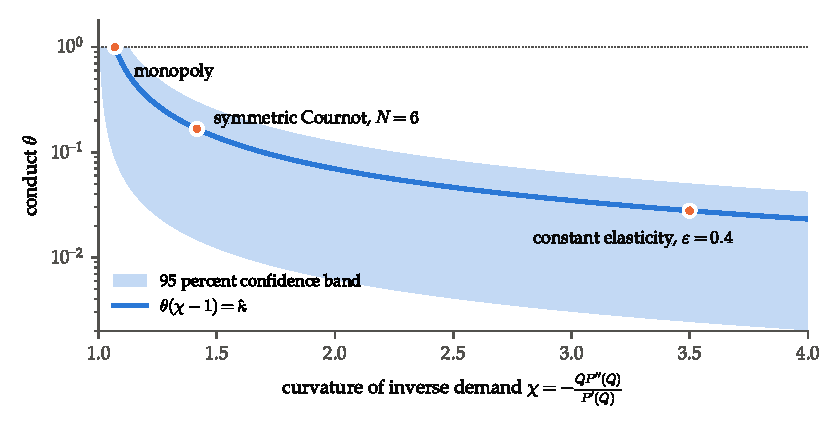
\includegraphics[width=0.9\textwidth]{figures/ch03/sumner_identified_set.pdf}
\caption{Pairs of demand curvature $\chi$ and conduct $\theta$ consistent with the estimated cigarette tax pass-through
$\hat\rho = 1.0746$. The curve is $\theta(\chi - 1) = \hat\kappa$ with $\hat\kappa = 0.069$, and the band maps the 95
percent state-clustered confidence interval for $\rho$. The marked points are monopoly ($\chi = 1.069$), symmetric
Cournot with six firms ($\chi = 1.42$, $\theta = \frac{1}{6}$) and constant-elasticity demand with $\varepsilon = 0.4$
($\chi = 3.5$, $\theta = 0.028$). The vertical axis is logarithmic.}
\label{fig:03-identified-set}
\end{figure}

\casehead{A bound that does not depend on curvature}
Outside information on the industry elasticity can rule out monopoly without any assumption on curvature. With flat
marginal cost $c \ge 0$ and tax $t$, the Lerner form of \eqref{eq:03-supply-tax} is
$\frac{P - t - c}{P} = \frac{\theta}{\varepsilon}$, where $\varepsilon$ is the elasticity at the observed equilibrium.
Since $c \ge 0$,
\begin{equation}\label{eq:03-lerner-bound}
\theta = \varepsilon\Bigl(1 - \frac{t}{P} - \frac{c}{P}\Bigr) \le \varepsilon\Bigl(1 - \frac{t}{P}\Bigr).
\end{equation}
The tax is a large share of the cigarette price. At the sample mean share of 0.467 and $\varepsilon = 0.4$, the bound
gives $\theta \le 0.213$. At the lowest share in the sample (0.229) it gives $\theta \le 0.308$. Both rule out monopoly.
Equivalently, monopoly at the mean tax share requires an elasticity of at least $\frac{1}{1 - 0.467} = 1.88$ at the
observed price. The bound uses the level of prices and taxes, and pass-through does not enter it. Sullivan's bound in
\cref{sec:03-sullivan} develops the same idea with an elasticity estimated from the tax variation itself.

\begin{remark}[Pass-through as a tool]\label{rem:03-passthrough-tool}
\Cref{prop:03-passthrough} turns pass-through into a measurement device. Given estimates of $\rho$, $\varepsilon$
and the slope of marginal cost, it pins down conduct for any assumed curvature. Conversely, given conduct, it predicts
the incidence of taxes and cost shocks. \citet{WeylFabinger2013} develop this program in general. Recent applications
combine first-order conditions of this kind with credible sources of variation. \citet{MillerOsborneSheu2017} study
the US portland cement industry from 1980 to 2010. Their estimated pass-through of fuel costs ranges from 1.03 to 1.65
across specifications (Table~4, p.~84). They combine it with conduct estimates from earlier work to measure the incidence
of a price on carbon emissions.
\citet{BergquistDinerstein2020} use the first-order-condition approach to estimate the effect of coordination among
intermediaries in the Kenyan maize market. Their field experiment supplies the instruments
\citep[p.~214, n.~86]{AskerNocke2021}.
Identification of conduct still requires curvature, which must come from demand estimated over a range of prices or
from assumption.
\end{remark}

\casehead{Contribution}
Sumner's paper introduced a design that is now standard. It uses an observed, exogenous component of marginal cost
and a fixed-effects panel to learn about the pricing rule without measuring cost. Its rejection of competition holds for
any demand curve and any non-decreasing marginal cost, although clustering weakens it. Its rejection of collusion holds
only given curvature, or given an industry elasticity and the curvature-free bound \eqref{eq:03-lerner-bound}. The
lesson extends beyond cigarettes. A market-wide cost shifter traces out demand and reveals the slope of perceived
marginal revenue, which mixes conduct with curvature. Cost shifters therefore deliver tests and bounds on conduct.
Point identification requires variation that rotates demand (\cref{sec:03-identification}), cost shifters specific to
one firm (\cref{sec:03-residual-demand}), or direct measures of cost (\cref{sec:03-sugar,sec:03-electricity}).
